\section{Summative and Formative
Evaluations}\label{summative-and-formative-evaluations}

The results were analyzed in two stages: (i) productivity analysis and
(ii) behavior analysis. The productivity analysis compares the
production performance of the two scheduling approaches, while the
behavior analysis explains how these results were achieved.

To compare the performance of the two scheduling methods, hypothesis
tests were conducted to determine whether there were statistically
significant differences (\colorbox{yellow!40}{\hyperref[_Ref187517011]{Figure 7}}).
Specifically, each test examined the null hypothesis that both
scheduling methods come from the same probability distribution. Because
at least one sample in each comparison failed the Shapiro--Wilk
(normality) or Levene (homoscedasticity) tests, the Wilcoxon test was
used instead of the two-sample t-test (Law, 2015; Telles \emph{et al.},
2020b). The Wilcoxon test was performed at a 95\% confidence level and a
5\% significance level (\colorbox{yellow!40}{}\hyperref[_Ref187517192]{Table 3}).

\begin{figure}[htbp]
\centering
\begin{subfigure}[b]{0.48\textwidth}
\centering
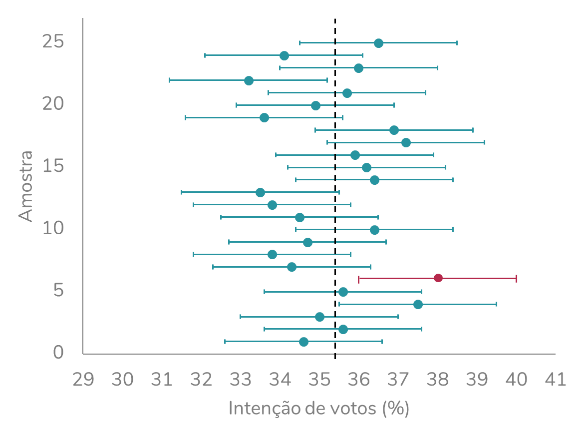
\includegraphics[width=\linewidth]{figures/fig07abcd.png}
\caption{}
\label{fig:sub:a}
\end{subfigure}
\begin{subfigure}[b]{0.48\textwidth}
\centering
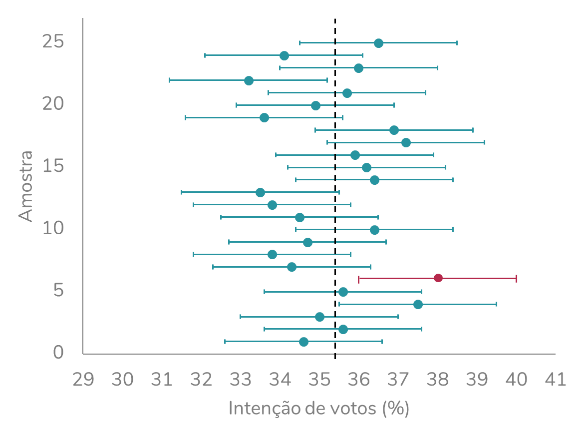
\includegraphics[width=\linewidth]{figures/fig07abcd.png}
\caption{}
\label{fig:sub:b}
\end{subfigure}
%
\begin{subfigure}[b]{0.48\textwidth}
\centering
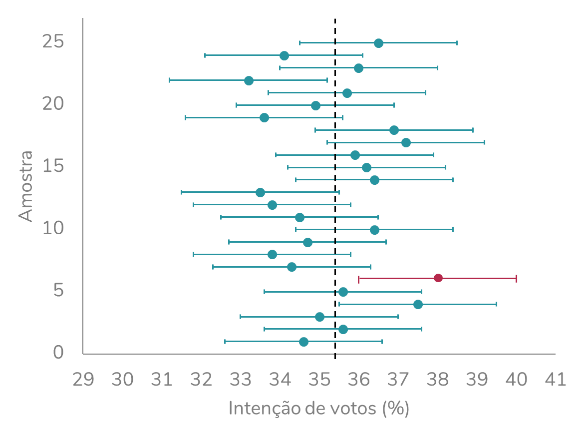
\includegraphics[width=\linewidth]{figures/fig07abcd.png}
\caption{}
\label{fig:sub:c}
\end{subfigure}
\begin{subfigure}[b]{0.48\textwidth}
\centering
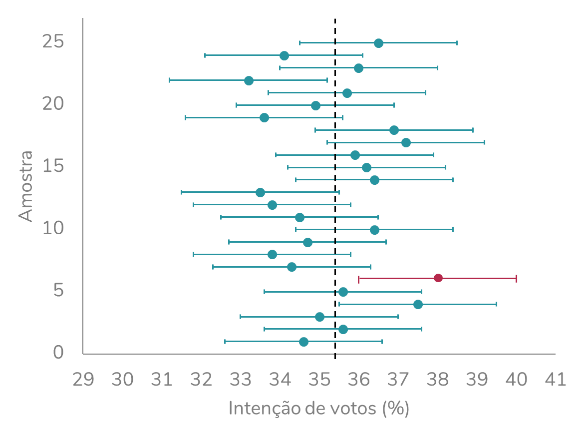
\includegraphics[width=\linewidth]{figures/fig07abcd.png}
\caption{}
\label{fig:sub:d}
\end{subfigure}
%
\caption{\protect\phantomsection\label{_Ref187517011}{}\colorbox{yellow!40}{Figure 7. Confidence
intervals of the differences for: (a) the number of products produced
and sold; (b) the average number of parts in process; (c) the average
level of the CB; and (d) the average level of the SB.}}
\end{figure}

The results indicate no statistically significant differences in demand
(DM) or quantity of products sold (SP), showing that both approaches met
demand equally. However, throughput time (FT), work in process (WIP),
finished goods (FG), and total inventory (IV) levels are lower under the
RL approach.

Behavioral analysis was conducted using three techniques to examine the
relationship between state variables and the scheduling decisions. The
first technique, Spearman's correlation, evaluates the monotonic
relationship between two quantitative variables without requiring
linearity (Barbosa and Azevedo, 2018; Xiao \emph{et al.}, 2015). The
correlation analysis shows that DBR exhibits a negative relationship
between FG and WIP for the same product, reflecting the DBR mechanism
that maintains the shipping buffer (SB) at its reference value
regardless of production stage, thus balancing FG and WIP. The FG and
WIP levels of different products behave similarly, except for products 7
and 9, which are unrestricted and released based on consumption. Actions
showed no significant correlations with state variables, apart from weak
correlations in products 2, 6, 7 (with FG), and product 9 (with WIP).
The RL agent reveals a similar pattern regarding the relationship
between FG and WIP, particularly for products 7 and 9 though the
correlation is weaker. This implies that while the RL agent also seeks
to balance FG and WIP, additional factors influence its decisions.
Unlike DBR, the RL agent exhibits weak to moderate negative correlations
between the action and the respective WIP (except for product 9). This
negative correlation suggests that the RL agent prioritizes releasing
materials when WIP is low, a behavior not observed in DBR. The results
from both correlations can be found in appendix.

The second approach used linear regression to identify the contribution
of WIP and FG on the quantity of products released by the scheduling
methods. A linear regression was run for each product, treating WIP and
FG as independent variables and the quantity of products released as the
dependent variable (full table in appendix). The result shows that the
DBR actions display a strong linear relationship with state variables,
with coefficients of determination exceeding 80\%. The primary
influencing factors are the product's own WIP and FG levels, while the
constraint buffer (CB) has no discernible impact. RL shows lower
coefficients of determination, below 55\%. Although WIP and FG remain
the key decision variables, the influence of CB is again negligible.
However, RL's decisions are less strongly determined by WIP and FG than
DBR's, indicating additional complexities in the agent's decision-making
process.

To complement the analysis and make RL decisions readable, a Decision
Tree model was trained for each action based on the RL agent's
state--action history. In DBR, WIP and FG collectively account for more
than 85\% of the decision's explanatory power. In the RL agent, WIP
exerts more influence than FG, but combined they explain less than 50\%
of the decision-making process for each action
(\colorbox{yellow!40}{}\hyperref[_Ref187517031]{Figure 8}). Unlike DBR, where other
products' variables have minimal effect, several RL actions show up to
5\% influence from variables related to other products, underscoring a
more nuanced decision process.

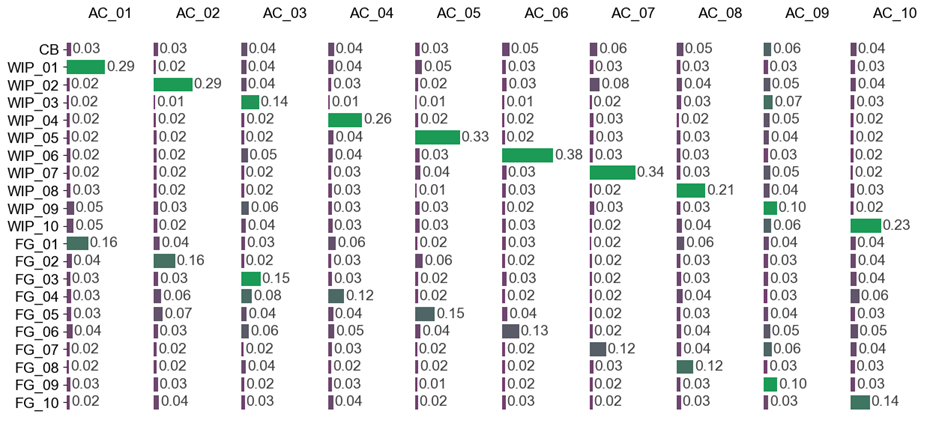
\includegraphics[width=6.30069in,height=2.9in]{figures/fig08.png}

\protect\phantomsection\label{_Ref187517031}{}Figure 8. Decision tree
influence of variables on RL actions

The number of nodes in a decision tree reflects how many rules are
required to explain the dataset (Myles \emph{et al.}, 2004; Rudin
\emph{et al.}, 2022). In this study, the DBR decision trees use fewer
nodes than their RL counterparts (\colorbox{yellow!40}{}\hyperref[_Ref187517024]{Figure
9}) indicating that the RL scheduling approach makes more complex
decisions. For DBR, products 7 and 9 exhibit the simplest trees because
they are not processed by the constraint, so their material release
depends only on the respective shipping buffer (SB). Conversely,
products 8 and 10 have the most complex trees, consistent with the fact
that they pass through the constraint and involve more processing steps.
In contrast, the RL decision trees do not show a clear pattern relating
the number of nodes to the model's dynamics. Notably, product 9 has the
largest tree in RL's case, despite not being processed by the
constraint.

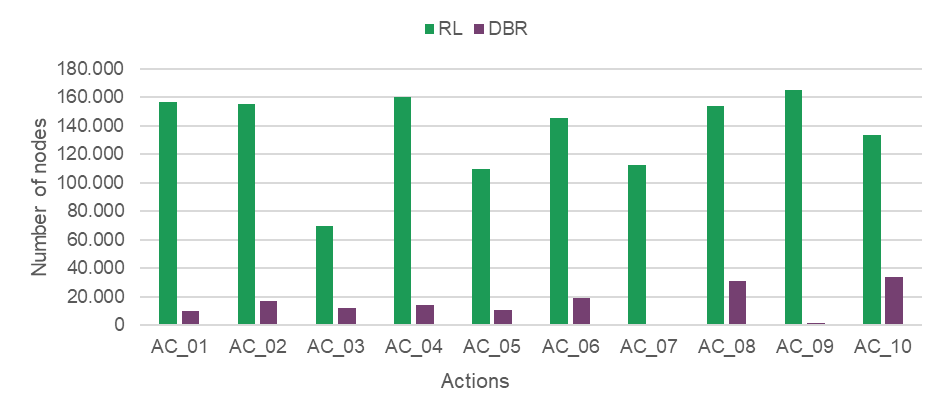
\includegraphics[width=6.30069in,height=2.76042in]{figures/fig09.png}

\protect\phantomsection\label{_Ref187517024}{}Figure 9. Quantity of
decision tree nodes.
